%% LyX 2.2.3 created this file.  For more info, see http://www.lyx.org/.
%% Do not edit unless you really know what you are doing.
\documentclass[oneside,english]{extbook}
\usepackage[T1]{fontenc}
\usepackage[latin9]{inputenc}
\usepackage{geometry}
\geometry{verbose,tmargin=25mm,bmargin=25mm,lmargin=25mm,rmargin=25mm}
\setcounter{secnumdepth}{3}
\setcounter{tocdepth}{3}
\setlength{\parindent}{0bp}
\synctex=1
\usepackage{babel}
\usepackage{float}
\usepackage{graphicx}
\usepackage{setspace}
\onehalfspacing
\usepackage[unicode=true,pdfusetitle,
 bookmarks=true,bookmarksnumbered=false,bookmarksopen=false,
 breaklinks=false,pdfborder={0 0 1},backref=false,colorlinks=false]
 {hyperref}

\makeatletter
%%%%%%%%%%%%%%%%%%%%%%%%%%%%%% User specified LaTeX commands.
\usepackage{amssymb}
\usepackage{color}
\usepackage{listings}
\definecolor{hellgelb}{rgb}{1,1,0.85}
\definecolor{colKeys}{rgb}{0,0,1}
\definecolor{colIdentifier}{rgb}{0,0,0}
\definecolor{colComments}{rgb}{1,0,0}
\definecolor{colString}{rgb}{0,0.5,0}
\lstset{
      language=Matlab,
      float=hbp,
      basicstyle=\footnotesize\ttfamily,
      identifierstyle=\color{colIdentifier},
      keywordstyle=\color{colKeys},
      stringstyle=\color{colString},
      commentstyle=\itshape\color{colComments},
      columns=fixed,
      tabsize=4,
      frame=single,
      framerule=1pt,
      extendedchars=true,
      showspaces=false,
      showstringspaces=false,
      numbers=left,
      numberstyle=\tiny\ttfamily,
      numbersep=1em,
      breaklines=true,
      breakindent=10pt,
      backgroundcolor=\color{hellgelb},
      breakautoindent=true,
      captionpos=t,
      xleftmargin=1em,
      xrightmargin=\fboxsep
}
\usepackage{lscape}
\usepackage{amsmath}
\usepackage{mathtools}
\usepackage{pifont}
\usepackage{color}
\usepackage{accents}

\delimitershortfall=-1pt
\let\Right\right
\let\Left\left
\makeatletter
\def\right#1{\Right#1\@ifnextchar){\!\right}{}}
\def\left#1{\Left#1\@ifnextchar({\!\left}{}}
\makeatother

\makeatother

\begin{document}
\pagenumbering{gobble}

\textbf{How many landmarks does the ONLINE SLAM algorithm need to
have a good performance?}

There's no simple answer. If there are a few landmarks then the landmark
assignment is good because if there's only few it's hard to confuse
them. On the other hand it means for the localization that if there
are only a few landmarks the algorithm has less observations to work
with, so the accuracy is low or even if there are too few landmarks
there can be parts in the trajectory without observations at all and
the algorithm only runs the prediction, therefore the pose uncertainty
will grow quickly. In conversely, if there are many landmarks then
localization is good, however, it's easy to confuse them. In order
to have many landmarks for good localization and still not to confuse
them the algorithm needs distinct landmarks.

\begin{figure}[H]
\centering{}\centering\includegraphics[scale=0.8]{../FIGURES/fig50}
\end{figure}

In our case all landmarks were the same because in the real world
they actually had exactly the same dimensions. But in practice the
landmarks may be different among them in different ways. For example,
it is very usual that they differ in dimensions or in color. Therefore,
if the algorithm uses the camera in addition it would have been able
to detect the different colors of our landmarks and then it could
have added the color as a component in the description of the landmarks.
But there are other features that can be used to distinguish the landmarks.
It can be the dimensions of the landmark, it can be a detector that
detects if a surface is flat or that detects the curvature of a surface
or that detects if there is a dihedral latch or even if there's a
corner. A camera can be used to detect an image of the object, so
the algorithm is able to detect feature points for which it can derive
a high dimensional vector. In general, the idea is to use landmark
signatures, so that each landmark is described by its position and
also its signature.

\begin{figure}[H]
\centering{}\centering\includegraphics[scale=0.8]{../FIGURES/fig51}
\end{figure}

Now our algorithm worked in the following way: The robot takes a scan
from the world. Then the algorithm detects the observed cylinders
in the scan and then it looks within a certain fixed radius for the
closest landmark. If there isn't a match between a cylinder and a
landmark the algorithm creates a new landmark. In our experiments
we used a radius of 50 cm, then a radius of 40 cm and also a radius
of 30 cm and we found out that the algorithm is brittle with respect
to this parameter.

Now let's think about how to make the landmark assignment process
more robust and reliable. Imagine the following situation. The robot
measures the cylinder labeled as A and the cylinder labeled as B.
In our map there is a landmark labeled as A' that the robot has observed
very often. Consequently, the uncertainty ellipse for the landmark
A' is pretty small. On the other hand, there is also a landmark labeled
as B', which is a bit further away from cylinder B, than the distance
from landmark A' to cylinder A. Besides, the uncertainty ellipse for
the landmark B' is really large.

Obviously the cylinder A shouldn't be assigned to landmark A'. Let's
explain this. The uncertainty ellipse for the landmark A' is really
small, due to the fact that the robot has observed this landmark many
times, so it means that the landmark A' is very well positioned in
the world. If the cylinder A is not very very close to the landmark
A', which is very well positioned in the world, is because, it's very
sure that there is another landmark next to the cylinder A.
\begin{center}
(Note that we haven't talked about radius to do the assignment yet)
\par\end{center}

On the other hand, the cylinder B should be assigned to the landmark
B'. The uncertainty ellipse for the landmark B' is really large, so
it means that the landmark B' couldn't be properly positioned in the
world. In this occasion, and due to the large uncertainty ellipse
for the landmark B', the cylinder B is considered to be close enough
to this landmark to be assigned to it.

The landmark assignment process should take into account the uncertainty
of the robot as well.

\begin{figure}[H]
\centering{}\centering\includegraphics[scale=0.8]{../FIGURES/fig53}
\end{figure}

The new landmark assignment process is called\textbf{ maximum likelihood
landmark} assignment and is based on the Mahalanobis distance. The
general expression for the squared Mahalanobis distance between any
measurement, $\vec{z}_t$, and the expected measurement to any world
landmark, $\vec{\hat{z}}_t\,=\,h\left(\vec{x}_t,\,\vec{p}_W\right)$,
is:

\begin{gather*}
M_{t}^2\,=\,\left(\vec{z}_t\,-\,\vec{\hat{z}}_{t}\right)^T\,\cdot\, Q_{t}^{-1}\,\cdot\,\left(\vec{z}_t\,-\,\vec{\hat{z}}_{jt}\right)\\
Q_{jt}\,=\, H_{t}\,\cdot\,\overline{\Sigma}_t\,\cdot\, H_{t}^T\,+\, Q
\end{gather*}

where the term $\vec{p}_W$ represents the coordinates of a world
landmark:

\begin{align*}
\vec{p}_W\,=\,\begin{pmatrix}
x_W\\
y_W
\end{pmatrix}
\end{align*}

Let's denote $M_{jt}^2$ to the squared Mahalanobis distance between
any measurement, $\vec{z}_t$, and the expected measurement to the
world landmark number $j,\,\vec{\hat{z}}_{jt}\,=\,h\left(\vec{\overline{\mu}}_{t},\,{\vec{\overline{p}}_W}_j\right)$:

\begin{gather*}
M_{jt}^2\,=\,\left(\vec{z}_t\,-\,\vec{\hat{z}}_{jt}\right)^T\,\cdot\, Q_{jt}^{-1}\,\cdot\,\left(\vec{z}_t\,-\,\vec{\hat{z}}_{jt}\right)\\
Q_{jt}\,=\, H_{jt}\,\cdot\,\overline{\Sigma}_t\,\cdot\, H_{jt}^T\,+\, Q
\end{gather*}

where the term ${\vec{\overline{p}}_W}_j$ represents the predicted
coordinates for the world landmark number $j$:

\begin{align*}
{\vec{\overline{p}}_W}_j\,=\,\begin{pmatrix}
\overline{\mu}_{{x_W}_j}\\
\overline{\mu}_{{y_W}_j}
\end{pmatrix}
\end{align*}

Finally, let's denote $M_{jit}^2$ to the squared Mahalanobis distance
between the measurement number $i$, $\vec{z}_{it}$, and the expected
measurement to the world landmark number $j,\,\vec{\hat{z}}_{jt}\,=\,h\left(\vec{\overline{\mu}}_{t},\,{\vec{\overline{p}}_W}_j\right)$:

\begin{gather*}
M_{jit}^2\,=\,\left(\vec{z}_{it}\,-\,\vec{\hat{z}}_{jt}\right)^T\,\cdot\, Q_{jt}^{-1}\,\cdot\,\left(\vec{z}_{it}\,-\,\vec{\hat{z}}_{jt}\right)\\
Q_{jt}\,=\, H_{jt}\,\cdot\,\overline{\Sigma}_t\,\cdot\, H_{jt}^T\,+\, Q
\end{gather*}

The subscript $j$ is the number of the registered world landmark
that the algorithm is currently using. The predicted $x$ coordinate
for the world landmark number $j$, $\overline{\mu}_{{x_W}_j}$, is
stored within the predicted state vector, $\vec{\overline{\mu}}_t$,
at the index:

\[
i\,=\,3\,+\,(2\,j)\,-\,1
\]

The predicted $y$ coordinate for the world landmark number $j$,
$\overline{\mu}_{{y_W}_j}$, is stored within the predicted state
vector, $\vec{\overline{\mu}}_t$, at the index

\[
i\,=\,3\,+\,(2\,j)
\]

\begin{align*}
\vec{\overline{\mu}}_t\,=\,\begin{pmatrix}
\overline{\mu}_{x_t}\\
\overline{\mu}_{y_t}\\
\overline{\mu}_{\theta_t}\\
\overline{\mu}_{{x_W}_1}\\
\overline{\mu}_{{y_W}_1}\\
\vdots\\
\overline{\mu}_{{x_W}_j}\\
\overline{\mu}_{{y_W}_j}\\
\vdots\\
\overline{\mu}_{{x_W}_N}\\
\overline{\mu}_{{y_W}_N}\\
\end{pmatrix}\begin{matrix*}[l]
\longleftarrow i\,=\,0\\
\longleftarrow i\,=\,1\\
\longleftarrow i\,=\,2\\
\textcolor{white}{\overline{\mu}_{{x_W}_1}}\\
\textcolor{white}{\overline{\mu}_{{y_W}_1}}\\
\textcolor{white}{\vdots}\\
\longleftarrow\text{Predicted $x$ coordinated for the world landmark number $j$, } i\,=\, 3\,+\,(2\,j)\,-\,1\\
\longleftarrow\text{Predicted $y$ coordinated for the world landmark number $j$, } i\,=\, 3\,+\,(2\,j)\\
\textcolor{white}{\vdots}\\
\textcolor{white}{\overline{\mu}_{{x_W}_N}}\\
\textcolor{white}{\overline{\mu}_{{y_W}_N}}
\end{matrix*}
\end{align*}

The observation vector, $\vec{z}_t$, is comprises by two terms:

\begin{align*}
\vec{z}_t\,=\,\begin{pmatrix}
D_t\\
\phi_t
\end{pmatrix}
\end{align*}

The term $D_t$ is the distance from the laser scanner to a detected
landmark.

The term $\phi_t$ is the angle defined between the laser scanner's
longitudinal axis and the imaginary line that joints the laser scanner
with a detected landmark.

\begin{figure}[H]
\centering\includegraphics[scale=0.95]{../FIGURES/fig55}
\end{figure}

The expected observation vector, $\vec{\hat{z}}_{jt}\,=\,h\left(\vec{\overline{\mu}}_t,\, {\vec{p}_W}_j\right)$,
is comprises by two terms:\begin{align*}
\vec{\hat{z}}_{jt}\,=\,\begin{pmatrix}\hat{D}_{jt}\\\hat{\phi}_{jt}\end{pmatrix}
\end{align*}

The term $\hat{D}_{jt}$ is the distance from the laser scanner's
predicted pose, $\vec{\overline{\mu}}_{lt}^{\,T}\,=\,\left(\overline{\mu}_{x_{lt}},\,\overline{\mu}_{y_{lt}},\,\overline{\mu}_{\theta_{t}}\right)$,
to the predicted position for the registered world landmark number
$j$, $\left(\overline{\mu}_{{x_W}_j},\,\overline{\mu}_{{y_W}_j}\right)$.

\begin{gather*}
\hat{D}_{jt}\,=\,\sqrt{\left(\overline{\mu}_{{x_W}_j}\,-\,\overline{\mu}_{x_{lt}}\right)^2\,+\,\left(\overline{\mu}_{{y_W}_j}\,-\,\overline{\mu}_{y_{lt}}\right)^2}\\
\overline{\mu}_{x_{lt}}\, =\,\overline{\mu}_{x_t}\, +\, sd\,\cos\left(\overline{\mu}_{\theta_t}\right)\\
\overline{\mu}_{y_{lt}}\, =\,\overline{\mu}_{y_t}\, +\, sd\,\sin\left(\overline{\mu}_{\theta_t}\right)
\end{gather*}

The term $\hat{\phi}_{jt}$ is the angle between:
\begin{itemize}
\item The laser scanner's predicted orientation angle, $\overline{\mu}_{\theta_t}$
and
\item The orientation angle of the imaginary line that joints the laser
scanner's predicted position with the predicted position for the registered
world landmark number $j$, $\arctan\left(\dfrac{\overline{\mu}_{{y_W}_j}\,-\,\overline{\mu}_{y_{lt}}}{\overline{\mu}_{{x_W}_j}\,-\,\overline {\mu}_{x_{lt}}}\right)$
\end{itemize}
\begin{align*}
\hat{\phi}_{jt}\,=\,\arctan\left(\dfrac{\overline{\mu}_{{y_W}_j}\,-\,\overline{\mu}_{y_{lt}}}{\overline{\mu}_{{x_W}_j}\,-\,\overline{\mu}_{x_{lt}}}\right)\,-\,\overline{\mu}_{\theta_t}
\end{align*}

\begin{figure}[H]
\centering\includegraphics[scale=0.95]{../FIGURES/fig57}
\end{figure}

Note:

The difference

\begin{align*}
\vec{z}_t\,-\,\vec{\hat{z}}_{jt}
\end{align*}

is a measurement of how well the detected landmark matches with the
registered world landmark number $j$.

The matrix $Q$ is the covariance matrix due to the uncertainty (error)
produced in the measure system. The matrix $\overline{\Sigma}_t$
is the uncertainty (error) in the predicted state vector, $\vec{\overline{\mu}}_t$.
By multiplying the matrix $\overline{\Sigma}_t$ from the left by
the term $H_{jt}$, and from the right by the term $H_{jt}^T$, the
algorithm is propagating the uncertainty (error) through the function
$h\left(\vec{x}_t,\, \vec{p}_W\right)$. Therefore, the term $H_{jt}\,\cdot\,\overline{\Sigma}_t\,\cdot\, H_{jt}^T$
represents the uncertainty propagation. Basically this term is due
to the uncertainty (error) in the robot's predicted pose and the uncertainty
in the measure system.

Then the algorithm uses a maximum distance threshold, $\epsilon$,
to accept the match between the detected landmark number $i$ and
the registered world landmark number $j$. The match is accepted or
rejected based on the squared Malahanobis distance.

\begin{gather*}
M_{jit}^2\,\leq\,\epsilon\\
\left(\vec{z}_{it}\,-\,\vec{\hat{z}}_{jt}\right)^T\,\cdot\, Q_{jt}^{\,-1}\,\cdot\,\left(\vec{z}_{it}\,-\,\vec{\hat{z}}_{jt}\right)\,\leq\,\epsilon
\end{gather*}

If $M_{jit}^2\,\leq\,\epsilon$ then the algorithm accepts the match
between the detected landmark number $i$ and the registered world
landmark number $j$. Otherwise, the match is rejected.

What is happening here is that:

\emph{The algorithm is accepting the match between the detected landmark
$i$ and the world landmark number $j$ if the measurement $\vec{z}_{it}$
is inside, or in the border, of the projection ellipse defined by
$\left(\vec{z}_{t}\,-\,\vec{\hat{z}}_{jt}\right)^T\,\cdot\,Q_{jt}^{\,-1}\,\cdot\,\left(\vec{z}_{t}\,-\,\vec{\hat{z}}_{jt}\right)\,=\,\epsilon$.}

This projection ellipse belongs to the Gaussian distribution $\mathcal{N}\left(\vec{z}_t,\,\vec{\hat{z}}_{jt},\, Q_{jt}\right)$.

\begin{figure}[H]
\centering{}\centering\includegraphics[scale=0.95]{../FIGURES/fig59}
\end{figure}

The projection ellipse is centered at the vector $\vec{\hat{z}}_{jt}\,=\,h\left(\vec{\overline{\mu}}_t,\, {\vec{\overline{p}}_W}_j\right)$.
The projection ellipse is oriented according to the orthonormal eigenvectors
of the covariance matrix $Q_{jt}$. The principal axes' lengths of
the projection ellipse depend on the eigenvalues of the covariance
matrix $Q_{jt}$, $\sqrt{\epsilon\,\lambda_1}$ and $\sqrt{\epsilon\,\lambda_2}$.

\begin{figure}[H]
\centering{}\centering\includegraphics[scale=0.95]{../FIGURES/fig60}
\end{figure}

Regarding the landmark assignment, now, there is also a provisional
landmark list. Let's consider that the robot sees a landmark for the
first time. Now the algorithm will not put this landmark into the
specific state vector as a standard landmark. Rather the algorithm
will store that landmark in the provisional landmark list and it will
add to the covariance matrix the landmark's position variances. The
robot moves on and it observes the landmark again (for the second
time), therefore the landmark uncertainty ellipse will decrease.

\begin{figure}[H]
\centering\includegraphics[scale=0.95]{../FIGURES/fig61}
\end{figure}

The algorithm will put the landmark into the final landmark list only
after several observations indicate that this landmark has been found
consistently.

\begin{figure}[H]
\centering\includegraphics[scale=0.95]{../FIGURES/fig62}
\end{figure}

In practice, it is relatively easy to handle this. The idea is that
any newly observed landmark is considered provisional and it is stored
into the specific state vector. But the observation model is modified
in a way that for provisional landmarks this model only handles the
position of these landmark as variables (concept of mathematics variable)
and the robot's position and orientation are not consider as variables.
In this way as long as a landmark is considered provisional the robot
will influence, by subsequent observations, the accuracy of that provisional
landmark's position but that provisional landmark won't influence
the robot's pose. So the algorithm adds a flag to know whether a landmark
is considered provisional or not, and therefore it can be used a slightly
different observation model.

\textbf{OVERVIEW:}
\begin{itemize}
\item \textbf{FULL SLAM problem}: the algorithm computes the posterior over
all states and assignments of landmarks. This problem is usually computationally
infeasible.
\item \textbf{ONLINE SLAM problem}: this problem is easier to handle and
it uses a deterministic computation of landmark assignments so instead
of providing the full posterior over all states and assignments you
sign on the fly using a deterministic algorithm. This is also its
main drawback because as we saw it's brittle with respect to landmark
confusion. Even though the ONLINE SLAM is less complex than the full
slam it still has a huge update complexity that grows with the number
of landmarks because the size of the specific state vector grows with
a number of landmarks so it is potentially unbound. Nevertheless ONLINE
SLAM has been used by many groups with considerable success and as
you have seen for a small problem it has worked out perfectly.
\end{itemize}
\begin{figure}[H]
\centering\includegraphics[scale=0.95]{../FIGURES/fig63}
\end{figure}

\end{document}
